\documentclass[]{article}

\usepackage[left=2.00cm, right=2.00cm, top=2.00cm, bottom=2.00cm]{geometry}
\usepackage[spanish,es-noshorthands]{babel}
\usepackage[utf8]{inputenc} % para tildes y ñ
\usepackage{graphicx} % para las figuras
\usepackage{xcolor}
\usepackage{listings} % para el código fuente en c++

\lstdefinestyle{customc}{
  belowcaptionskip=1\baselineskip,
  breaklines=true,
  frame=single,
  xleftmargin=\parindent,
  language=C++,
  showstringspaces=false,
  basicstyle=\footnotesize\ttfamily,
  keywordstyle=\bfseries\color{green!40!black},
  commentstyle=\itshape\color{gray!40!gray},
  identifierstyle=\color{black},
  stringstyle=\color{orange},
}
\lstset{style=customc}


%opening
\title{Práctica 3. Divide y vencerás}
\author{David Luna Jurado \\ % mantenga las dos barras al final de la línea y este comentario
david.lunajurado@alum.uca.es\\ % mantenga las dos barras al final de la linea y este comentario
Teléfono: 663590384 \\ % mantenga las dos barras al final de la línea y este comentario
NIF: 32098835N \\ % mantenga las dos barras al final de la línea y este comentario
}


\begin{document}

\maketitle

%\begin{abstract}
%\end{abstract}

% Ejemplo de ecuación a trozos
%
%$f(i,j)=\left\{ 
%  \begin{array}{lcr}
%      i + j & si & i < j \\ % caso 1
%      i + 7 & si & i = 1 \\ % caso 2
%      2 & si & i \geq j     % caso 3
%  \end{array}
%\right.$

\begin{enumerate}
\item Describa las estructuras de datos utilizados en cada caso para la representación del terreno de batalla. 

El valor de las celdas para la colocación del extractor de minerales se realiza calculando la distancia de dicha casilla respecto al centro.
El valor de la casilla será el inverso de la distancia, de esta forma las casillas más cercanas al centro tendrán más valor.

% Elimine los símbolos de tanto por ciento para descomentar las siguientes instrucciones e incluir una imagen en su respuesta. La mejor ubicación de la imagen será determinada por el compilador de Latex. No tiene por qué situarse a continuación en el fichero en formato pdf resultante.
\begin{figure}
\centering
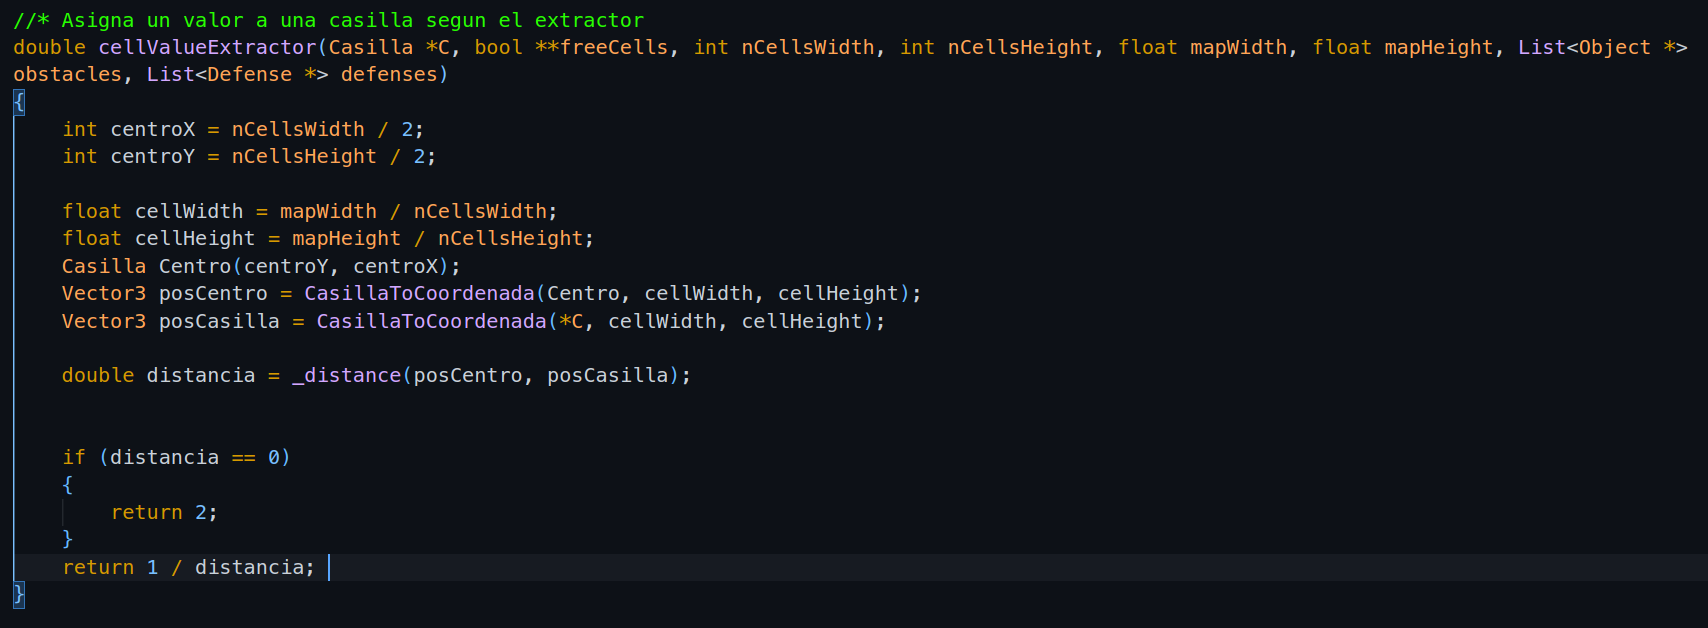
\includegraphics[width=0.7\linewidth]{./CellValueExtractor.png} % no es necesario especificar la extensión del archivo que contiene la imagen
\caption{Estrategia devoradora para la mina}
\label{fig:defenseValueCellsHead}
\end{figure}

\item Implemente su propia versión del algoritmo de ordenación por fusión. Muestre a continuación el código fuente relevante. 

\begin{lstlisting}
void ordenacionInsercion(int *v, int i, int j)
{
    int aux = 0;
    int k;
    for (int l = i + 1; l <= j; l++)
    {
        bool colocado = false;
        int m = l;
        for (k = l - 1; k >= i && !colocado; k--)
        {
            if (v[m] > v[k])
            {
                aux = v[k];
                v[k] = v[m];
                v[m] = aux;
                m--;
            }
        }
    }
}
void fusion(int *v, int *w, int i, int k, int j)
{
    int n = j - i + 1;
    int p = i;
    int q = k + 1;
    for (int l = 0; l < n; l++)
    {
        if (p <= k && (q > j || v[p] > v[q]))
        {
            w[l] = v[p];
            p = p + 1;
        }
        else
        {
            w[l] = v[q];
            q = q + 1;
        }
    }

    for (int l = 0; l < n; l++)
    {
        v[i + l] = w[l];
    }
}
void ordenacionFusion(int *v, int *w, int i, int j)
{
    int n = j - i + 1;
    if (n <= 3)
    {
        ordenacionInsercion(v, i, j);
    }
    else
    {
        int k = i - 1 + n / 2;
        ordenacionFusion(v, w, i, k);
        ordenacionFusion(v, w, k + 1, j);
        fusion(v, w, i, k, j);
    }
}


void ordenacionRapida(int *v, int i, int j)
{
    int n = j - i + 1;
    if (n <= 3)
    {
        ordenacionInsercion(v, i, j);
    }
    else
    {
        int p = pivote(v, i, j);
        ordenacionRapida(v, i, p - 1);
        ordenacionRapida(v, p + 1, j);
    }
}

\end{lstlisting}


\item Implemente su propia versión del algoritmo de ordenación rápida. Muestre a continuación el código fuente relevante. 

\begin{lstlisting}
// sustituya este codigo por su respuesta
void placeDefenses(...) {

    List<Defense*>::iterator currentDefense = defenses.begin();
    while(currentDefense != defenses.end() && maxAttemps > 0) {

        (*currentDefense)->position.x = ((int)(_RAND2(nCellsWidth))) * cellWidth + cellWidth * 0.5f;
        ...
        ++currentDefense;
    }
}
\end{lstlisting}

\item Realice pruebas de caja negra para asegurar el correcto funcionamiento de los algoritmos de ordenación implementados en los ejercicios anteriores. Detalle a continuación el código relevante.

El conjunto de Candidatos son las casillas.
\newline
El conjunto de Candidatos seleccionados son las casillas en las que se coloca una defensa.
\newline
La función solucion en este caso es !Colocadas[0], que nos indicará si se ha colocado el extractor o no.
\newline
La función de selección: CasillasExtractor.front() Debido a que la lista de Casillas está ordenada.
\newline
La función de factibilidad de corresponde a esFactible(seleccionada, freeCells, cellWidth, cellHeight, mapWidth, mapHeight, obstacles, defenses, *centroDeExtraccion, Colocadas)
\newline
La función objetivo es cellValueExtractor(\&C, freeCells, nCellsWidth, nCellsHeight, mapWidth, mapHeight, obstacles, defenses);
Que asigna valor a las casillas.
El objetivo es maximizar el tiempo que duran las defensas en batalla.

\item Analice de forma teórica la complejidad de las diferentes versiones del algoritmo de colocación de defensas en función de la estructura de representación del terreno de batalla elegida. Comente a continuación los resultados. Suponga un terreno de batalla cuadrado en todos los casos. 

El valor de las celdas para la colocación del extractor de minerales se realiza calculando la distancia de dicha casilla respecto al centro de extracción de minerales.
El valor de la casilla será el inverso de la distancia, de esta forma las casillas más cercanas al centro de extracción tendrán más valor.
Aunque se le dará más valor a las casillas que estén a una distancia de dos Casillas con respecto al centro de extracción, para asegurar que haya casillas con una distancia prudencial respecto al centro.


\item Incluya a continuación una gráfica con los resultados obtenidos. Utilice un esquema indirecto de medida (considere un error absoluto de valor 0.01 y un error relativo de valor 0.001). Es recomendable que diseñe y utilice su propio código para la medición de tiempos en lugar de usar la opción \emph{-time-placeDefenses3} del simulador. Considere en su análisis los planetas con códigos 1500, 2500, 3500,..., 10500, al menos. Puede incluir en su análisis otros planetas que considere oportunos para justificar los resultados. Muestre a continuación el código relevante utilizado para la toma de tiempos y la realización de la gráfica.

\begin{figure}[h]
    \centering
    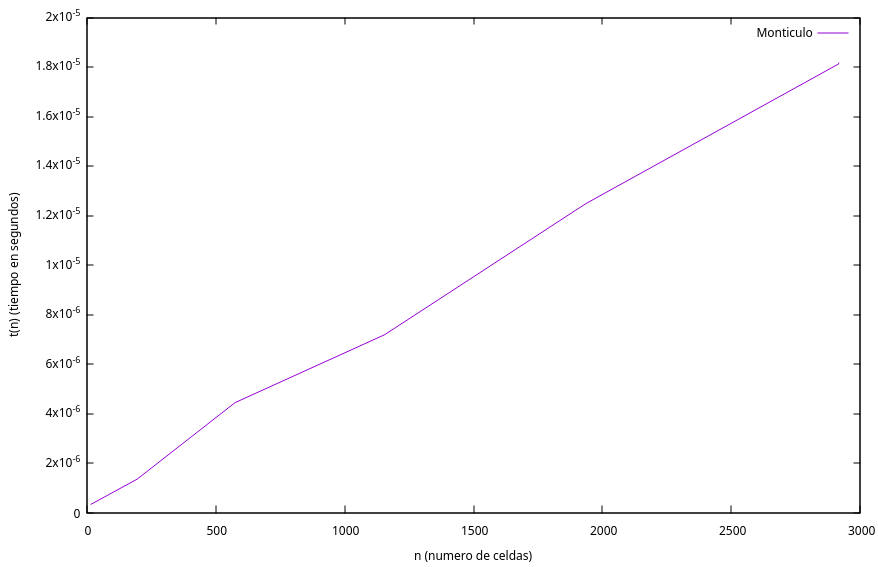
\includegraphics[width=10cm]{graphic.png}
    \label{fig:msf_nmap_ftp}
\end{figure}

\end{enumerate}

Todo el material incluido en esta memoria y en los ficheros asociados es de mi autoría o ha sido facilitado por los profesores de la asignatura. Haciendo entrega de este documento confirmo que he leído la normativa de la asignatura, incluido el punto que respecta al uso de material no original.

\end{document}
